\documentclass[9pt,a4paper]{extarticle}
\usepackage[a4paper,margin=9mm,top=8mm,bottom=10mm]{geometry}
% ===== Shared preamble: Class 12 Chemistry (project style, from physics-formula-sheet-source.tex) =====
\usepackage[T1]{fontenc}
\usepackage{lmodern}
\usepackage{amsmath,amssymb}
\usepackage{multicol}
\usepackage[most]{tcolorbox}
\usepackage{enumitem}
\usepackage{booktabs,tabularx,array}
\usepackage{fancyhdr}
\usepackage{xcolor}
\usepackage{microtype}
\usepackage[version=4]{mhchem}
\usepackage{tikz}
\usetikzlibrary{arrows.meta,calc}
\usepackage{pifont}
\usepackage{needspace}
\DeclareUnicodeCharacter{21CC}{\ensuremath{\rightleftharpoons}}
\DeclareUnicodeCharacter{2713}{\ding{51}}
\DeclareUnicodeCharacter{03B1}{\ensuremath{\alpha}}
\DeclareUnicodeCharacter{03B2}{\ensuremath{\beta}}
\DeclareUnicodeCharacter{2192}{\ensuremath{\to}}
\DeclareUnicodeCharacter{2610}{\ensuremath{\square}}
\DeclareUnicodeCharacter{21D2}{\ensuremath{\Rightarrow}}
\DeclareUnicodeCharacter{2194}{\ensuremath{\leftrightarrow}}
\DeclareUnicodeCharacter{2605}{\ding{72}}

% ---------- Colours: one per unit ----------
\definecolor{navy}{HTML}{1B2A4A}
\definecolor{uI}{HTML}{1F5FAD}    % 1 Solutions
\definecolor{uII}{HTML}{0E8A7E}   % 2 Electrochemistry
\definecolor{uIII}{HTML}{C2571A}  % 3 Chemical Kinetics
\definecolor{uIV}{HTML}{6A3FA0}   % 4 d- and f-Block
\definecolor{uV}{HTML}{B0204F}    % 5 Coordination Compounds
\definecolor{uVI}{HTML}{2E8B3A}   % 6 Haloalkanes & Haloarenes
\definecolor{uVII}{HTML}{8A6D00}  % 7 Alcohols, Phenols, Ethers
\definecolor{uVIII}{HTML}{2B6F8F} % 8 Aldehydes, Ketones, Acids
\definecolor{uIX}{HTML}{9A4A1E}   % 9 Amines
\definecolor{uX}{HTML}{5A5A5A}    % 10 Biomolecules
\definecolor{tipY}{HTML}{FFF4B8}
\definecolor{tipYframe}{HTML}{E0B400}
\definecolor{sqp}{HTML}{1B2A4A}
\colorlet{uc}{uI}

% ---------- Tag for questions in the official 2026-27 sample paper ----------
\newcommand{\tagbox}[2]{{\setlength{\fboxsep}{0.8pt}\colorbox{#1}{\textcolor{white}{\sffamily\bfseries\tiny\,#2\,}}}}
\newcommand{\SQP}{\tagbox{sqp}{SQP 26--27}}

% ---------- Unit banner & chapter bar ----------
\newcommand{\unitbanner}[3]{% colour, title, marks
  \colorlet{uc}{#1}%
  \par\vspace{2pt}\noindent
  \begin{tcolorbox}[enhanced,colback=#1,colframe=#1,arc=1.5pt,boxsep=1pt,left=4pt,right=4pt,top=1.5pt,bottom=1.5pt,before skip=2pt,after skip=2pt]
  \sffamily\bfseries\color{white}\footnotesize #2\hfill\scriptsize #3
  \end{tcolorbox}}
\newcommand{\chapbar}[1]{%
  \par\needspace{7\baselineskip}\noindent
  \begin{tcolorbox}[enhanced,colback=uc!18,colframe=uc,boxrule=0pt,leftrule=3pt,arc=0pt,boxsep=0.5pt,left=3pt,right=3pt,top=1pt,bottom=1pt,before skip=3pt,after skip=1.5pt]
  \sffamily\bfseries\color{uc!80!black}\footnotesize #1
  \end{tcolorbox}}
\newcommand{\sub}[1]{\par\needspace{4\baselineskip}\addvspace{2pt}\noindent{\sffamily\bfseries\scriptsize\color{uc}\strut\MakeUppercase{#1}}\par\vspace{0.5pt}}

% ---------- Boxes ----------
\newtcolorbox{kbox}{enhanced,colback=uc!5,colframe=uc,boxrule=0.6pt,arc=1.5pt,left=2pt,right=2pt,top=1pt,bottom=1pt,boxsep=1pt,before skip=2pt,after skip=2pt}
\newtcolorbox{tip}{enhanced,colback=tipY,colframe=tipYframe,boxrule=0.5pt,arc=1.5pt,left=2pt,right=2pt,top=0.5pt,bottom=0.5pt,boxsep=1pt,before skip=2pt,after skip=2pt,
  fontupper=\footnotesize}
\newtcolorbox{numbox}{enhanced,colback=white,colframe=uc!70,boxrule=0.5pt,arc=1.5pt,left=2pt,right=2pt,top=0.5pt,bottom=0.5pt,boxsep=1pt,before skip=2pt,after skip=2pt,
  borderline={0.4pt}{1.2pt}{uc!35,dashed}}
\newcommand{\Tip}{{\sffamily\bfseries\scriptsize TIP\;}}
\newcommand{\Num}{{\sffamily\bfseries\scriptsize\color{uc}STANDARD NUMERICALS\;}}

% ---------- Lists ----------
\setlist{nosep,leftmargin=8pt,labelsep=2pt}
\setlist[itemize]{label={\textcolor{uc}{\tiny$\blacktriangleright$}}}
\newenvironment{fl}{\begin{itemize}}{\end{itemize}}

% ---------- Mini graph helper (tikz) ----------
% \minigraph{width}{height}{x label}{y label}{drawing commands}
\newcommand{\minigraph}[5]{%
\begin{tikzpicture}[x=1cm,y=1cm,line cap=round,font=\tiny]
\draw[-{Stealth[length=3pt]},black!70] (0,0)--(#1,0) node[below left,inner sep=1pt]{#3};
\draw[-{Stealth[length=3pt]},black!70] (0,0)--(0,#2) node[above right,inner sep=1pt]{#4};
#5
\end{tikzpicture}}

\setlength{\columnsep}{9pt}
\setlength{\columnseprule}{0.3pt}
\def\columnseprulecolor{\color{black!25}}
\setlength{\parindent}{0pt}
\setlength{\abovedisplayskip}{1pt}\setlength{\belowdisplayskip}{1pt}
\setlength{\abovedisplayshortskip}{0pt}\setlength{\belowdisplayshortskip}{0pt}
\renewcommand{\arraystretch}{1.08}
\newcolumntype{Y}{>{\raggedright\arraybackslash}X}
\pagestyle{fancy}\fancyhf{}
\renewcommand{\headrulewidth}{0pt}

\fancyfoot[L]{\tiny\sffamily\color{black!55} Class 12 Chemistry · Formula \& Facts Sheet · Part 2: Inorganic Chemistry · CBSE Board 2026--27 (paper 27 Feb 2027)}
\fancyfoot[R]{\tiny\sffamily\color{black!55} Page \thepage}

% orbital boxes: 0 empty, 1 up, 2 pair, 3 ligand electron pair (shaded)
\newcommand{\ob}[1]{\begin{tikzpicture}[x=2.9mm,y=2.9mm,baseline=0.3mm,line width=0.35pt]
\foreach \s [count=\i from 0] in {#1}{%
 \ifnum\s=3 \fill[uc!28] (\i,0) rectangle ++(1,1);\fi
 \draw[black!65] (\i,0) rectangle ++(1,1);
 \ifnum\s>0 \draw[-{Stealth[length=1.6pt]}] (\i+0.33,0.12)--(\i+0.33,0.88);\fi
 \ifnum\s>1 \draw[{Stealth[length=1.6pt]}-] (\i+0.67,0.12)--(\i+0.67,0.88);\fi}
\end{tikzpicture}}
\newcommand{\obl}[1]{{\tiny #1}}

\raggedbottom
\begin{document}
\footnotesize

% ================= TITLE =================
\begin{tcolorbox}[enhanced,colback=navy,colframe=navy,arc=2pt,left=6pt,right=6pt,top=3pt,bottom=3pt]
\color{white}\sffamily
{\Large\bfseries Class 12 Chemistry — Formulas, Reactions \& Key Facts}\hfill{\small NCERT · Rationalised}\\[1pt]
{\footnotesize Part 2 of 3: \textbf{Inorganic Chemistry} (Ch 4--5) \;·\; CBSE Board 2026--27 only \;·\; Chemistry paper: \textbf{Sat 27 Feb 2027}}\\[2pt]
{\scriptsize Part 1 = Physical (Ch 1--3); Part 3 = Organic (Ch 6--10). \SQP\ = asked in the official CBSE 2026--27 sample paper.}
\end{tcolorbox}
\vspace{-1pt}
\noindent
\begin{tcolorbox}[enhanced,colback=navy!4,colframe=navy!60,boxrule=0.5pt,arc=1.5pt,left=3pt,right=3pt,top=1pt,bottom=1pt]
\scriptsize\sffamily\textbf{UNIT-WISE MARKS (70)}\rmfamily\quad
1 Solutions 7 · 2 Electrochem 9 · 3 Kinetics 7 · \textbf{\textcolor{uIV}{4 d- \& f-Block 7}} · \textbf{\textcolor{uV}{5 Coordination 7}} · 6 Haloalkanes 6 · 7 Alcohols 6 · 8 Carbonyls \& Acids 8 · 9 Amines 6 · 10 Biomolecules 7
\;→\; \textbf{Inorganic = 14 marks.}\quad
\sffamily\textbf{PAPER}\rmfamily\; A 16×1 (12 MCQ + 4 A--R) · B 5×2 · C 7×3 · D 2×4 case · E 3×5 · 3 h. Inorganic usually gives 3--5 MCQ/A--R, one or two 2/3-markers and often a case or 5-marker (naming + isomerism + VBT/CFT).\\
\sffamily\textbf{IN SYLLABUS}\rmfamily\; Ch 4: position, configuration, general properties, K$_2$Cr$_2$O$_7$ \& KMnO$_4$, lanthanoids, actinoids, applications. Ch 5: Werner, definitions, IUPAC naming, isomerism, VBT, CFT, metal carbonyls, importance \& applications. \textbf{Practical link:} KMnO$_4$ titrations vs oxalic acid and Mohr's salt.
\end{tcolorbox}

\begin{multicols}{2}\raggedcolumns
% =====================================================================
\unitbanner{uIV}{UNIT 4 · THE d- AND f-BLOCK ELEMENTS}{7 marks}
\chapbar{Position \& electronic configuration}
\begin{fl}
\item d-block: groups 3--12. Series: 3d (Sc--Zn), 4d (Y--Cd), 5d (La, Hf--Hg), 6d (Ac, Rf--Cn). General configuration $(n-1)d^{1-10}\,ns^{1-2}$ (Pd: $4d^{10}5s^0$).
\item \textbf{Transition element}: has an incompletely filled d subshell in the atom \emph{or} in any of its common oxidation states.
\item Zn, Cd, Hg ($d^{10}$ in atom and ions) are \emph{not} regarded as transition metals. Cu (Cu$^{2+}$ $3d^9$), Ag, Au (Au$^{3+}$ $5d^8$) \emph{are}. Sc is ($3d^1$).
\item Exceptions: Cr $3d^54s^1$, Cu $3d^{10}4s^1$ (extra stability of half-filled and full d).
\item Ions: remove 4s electrons first. Fe$^{2+}$ $3d^6$, Fe$^{3+}$ $3d^5$, Mn$^{2+}$ $3d^5$, Cu$^+$ $3d^{10}$.
\end{fl}
{\scriptsize\setlength{\tabcolsep}{2.2pt}
\begin{tabularx}{\linewidth}{@{}l l l Y c Y@{}}
\toprule
 & \textbf{Atom} & \textbf{M$^{2+}$} & \textbf{Common OS} & \textbf{$n$ (M$^{2+}$)} & \textbf{Aqua ion colour}\\
\midrule
Sc & $3d^14s^2$ & -- & +3 only & -- & Sc$^{3+}$ colourless\\
Ti & $3d^24s^2$ & $d^2$ & +4 (+3, +2) & 2 & Ti$^{3+}$ purple, Ti$^{4+}$ colourless\\
V & $3d^34s^2$ & $d^3$ & +5, +4, +3, +2 & 3 & V$^{4+}$ blue, V$^{3+}$ green, V$^{2+}$ violet\\
Cr & $3d^54s^1$ & $d^4$ & +3, +6 (+2) & 4 & Cr$^{3+}$ violet, Cr$^{2+}$ blue\\
Mn & $3d^54s^2$ & $d^5$ & +2 to +7 & 5 & Mn$^{2+}$ pink, Mn$^{3+}$ violet\\
Fe & $3d^64s^2$ & $d^6$ & +2, +3 & 4 & Fe$^{2+}$ green, Fe$^{3+}$ yellow\\
Co & $3d^74s^2$ & $d^7$ & +2, +3 & 3 & Co$^{2+}$ pink, Co$^{3+}$ blue\\
Ni & $3d^84s^2$ & $d^8$ & +2 & 2 & Ni$^{2+}$ green\\
Cu & $3d^{10}4s^1$ & $d^9$ & +2, +1 & 1 & Cu$^{2+}$ blue, Cu$^+$ colourless\\
Zn & $3d^{10}4s^2$ & $d^{10}$ & +2 only & 0 & Zn$^{2+}$ colourless\\
\bottomrule
\end{tabularx}\par}

\chapbar{General properties \& trends (3d series)}
\begin{fl}
\item \textbf{Metallic character}: hard, high m.p./b.p., high enthalpy of atomisation — strong metallic bonding from $(n-1)d$ + $ns$ electrons. Maximum near the middle (most unpaired d electrons). Mn and Zn lower; Hg is liquid. 4d/5d metals have higher $\Delta_aH$ than 3d (frequent metal--metal bonding in heavier metals).
\item \textbf{Radii}: decrease across the series, then stay nearly constant (added d electrons shield poorly). 4d and 5d radii almost equal (Zr 160 pm, Hf 159 pm) — lanthanoid contraction. Density rises Ti → Cu.
\item \textbf{Ionisation enthalpy}: rises gradually and irregularly. IE$_2$ high for Cr and Cu (would break $d^5$/$d^{10}$); IE$_3$ high for Mn and Zn (from $d^5$/$d^{10}$).
\item \textbf{Oxidation states}: variable because $(n-1)d$ and $ns$ energies are close; differ by one unit (Fe$^{2+}$/Fe$^{3+}$). Max OS rises to Mn (+7) and then falls. Mn shows the most OS. Highest OS appear in oxides/oxoanions (\ce{MnO4-}, \ce{Cr2O7^2-}) and fluorides; low/zero OS with $\pi$-acceptor ligands (\ce{Ni(CO)4}, \ce{Fe(CO)5}). Heavier members: higher OS more stable (Mo(VI), W(VI) vs oxidising Cr(VI)).
\item Highest Mn fluoride is MnF$_4$ but highest oxide Mn$_2$O$_7$ (+7): O forms multiple bonds with the metal.
\item \textbf{Oxides}: acidic character rises with OS. MnO basic, MnO$_2$ amphoteric, Mn$_2$O$_7$ acidic; CrO basic, Cr$_2$O$_3$ amphoteric, CrO$_3$ acidic; V$_2$O$_5$ amphoteric (mainly acidic).
\end{fl}
\sub{Standard electrode potentials (V)}
{\scriptsize\setlength{\tabcolsep}{2.4pt}
\begin{tabular}{@{}l*{9}{c}@{}}
\toprule
 & Ti & V & Cr & Mn & Fe & Co & Ni & Cu & Zn\\
\midrule
$E^\circ_{\ce{M^2+/M}}$ & $-1.63$ & $-1.18$ & $-0.90$ & $-1.18$ & $-0.44$ & $-0.28$ & $-0.25$ & $+0.34$ & $-0.76$\\
$E^\circ_{\ce{M^3+/M^2+}}$ & $-0.37$ & $-0.26$ & $-0.41$ & $+1.57$ & $+0.77$ & $+1.97$ & -- & -- & --\\
\bottomrule
\end{tabular}\par}
\begin{fl}
\item Cu alone has positive $E^\circ_{\ce{M^2+/M}}$: high $\Delta_aH$ + IE not balanced by $\Delta_\text{hyd}H$ → Cu does not liberate H$_2$ from acids.
\item Mn, Zn more negative than the trend: stable Mn$^{2+}$ ($d^5$), Zn$^{2+}$ ($d^{10}$). Ni: very negative $\Delta_\text{hyd}H$.
\item $E^\circ_{\ce{Mn^3+/Mn^2+}}$ high → Mn$^{3+}$ strong oxidant ($d^5$ Mn$^{2+}$ favoured). $E^\circ_{\ce{Cr^3+/Cr^2+}}$ negative → Cr$^{2+}$ strong reductant (Cr$^{3+}$ $t_{2g}^3$ stable). Fe$^{3+}$/Fe$^{2+}$ low → Fe$^{3+}$ ($d^5$) stable. Co$^{3+}$ unstable in water.
\end{fl}
\sub{Magnetic, colour, complexes, catalysis, interstitials, alloys}
\begin{kbox}
Spin-only moment: $\mu=\sqrt{n(n+2)}$ BM\quad($n$ = unpaired electrons)\\
$n=1$: 1.73 \;·\; 2: 2.83 \;·\; 3: 3.87 \;·\; 4: 4.90 \;·\; 5: 5.92 BM
\end{kbox}
\begin{fl}
\item Paramagnetic: unpaired electrons; diamagnetic: all paired ($d^0$, $d^{10}$).
\item \textbf{Colour}: d--d transition; ion absorbs part of visible light, we see the complementary colour. $d^0$ (Sc$^{3+}$, Ti$^{4+}$) and $d^{10}$ (Zn$^{2+}$, Cu$^+$) are colourless. (Purple \ce{MnO4-} and orange \ce{Cr2O7^2-} are $d^0$: colour from charge transfer.)
\item \textbf{Complexes}: small size, high ionic charge, vacant d orbitals of suitable energy.
\item \textbf{Catalysis}: variable OS and ability to form complexes / adsorb reactants on the surface. V$_2$O$_5$ (Contact process), finely divided Fe (Haber), Ni (hydrogenation). Fe$^{3+}$ catalyses \ce{S2O8^2-}/\ce{I-}: \ce{2Fe^3+ + 2I- -> 2Fe^2+ + I2}; \ce{2Fe^2+ + S2O8^2- -> 2Fe^3+ + 2SO4^2-}.
\item \textbf{Interstitial compounds}: small H, C, N, B trapped in metal lattice (TiC, Mn$_4$N, Fe$_3$H, TiH$_{1.7}$) — non-stoichiometric, very hard, high m.p., keep metallic conductivity, chemically inert.
\item \textbf{Alloys}: similar atomic radii → atoms substitute in the lattice (brass Cu--Zn, bronze Cu--Sn, steels).
\end{fl}

\chapbar{Potassium dichromate, K$_2$Cr$_2$O$_7$}
\begin{kbox}
From chromite: \ce{4FeCr2O4 + 8Na2CO3 + 7O2 -> 8Na2CrO4 + 2Fe2O3 + 8CO2}\\
\ce{2Na2CrO4 + 2H+ -> Na2Cr2O7 + 2Na+ + H2O};\quad \ce{Na2Cr2O7 + 2KCl -> K2Cr2O7 + 2NaCl}\\[1pt]
pH switch: \ce{2CrO4^2- + 2H+ <=> Cr2O7^2- + H2O}\; (yellow $\rightleftharpoons$ orange; base reverses it)\\[1pt]
Oxidant in acid: \ce{Cr2O7^2- + 14H+ + 6e- -> 2Cr^3+ + 7H2O}\; ($E^\circ=1.33$ V)
\end{kbox}
\begin{fl}
\item \ce{Cr2O7^2- + 14H+ + 6I- -> 2Cr^3+ + 3I2 + 7H2O}
\item \ce{Cr2O7^2- + 14H+ + 6Fe^2+ -> 2Cr^3+ + 6Fe^3+ + 7H2O}
\item \ce{Cr2O7^2- + 14H+ + 3Sn^2+ -> 2Cr^3+ + 3Sn^4+ + 7H2O}
\item \ce{Cr2O7^2- + 8H+ + 3H2S -> 2Cr^3+ + 3S + 7H2O}
\item Structure: chromate tetrahedral; dichromate = two tetrahedra sharing one O (Cr--O--Cr $\approx126^\circ$). Na$_2$Cr$_2$O$_7$ is more soluble; K$_2$Cr$_2$O$_7$ is used as a primary standard in volumetric analysis.
\end{fl}

\chapbar{Potassium permanganate, KMnO$_4$}
\begin{kbox}
\ce{2MnO2 + 4KOH + O2 -> 2K2MnO4 + 2H2O} (fusion);\quad \ce{3MnO4^2- + 4H+ -> 2MnO4- + MnO2 + 2H2O}\\
Commercial: alkaline manganate oxidised electrolytically \ce{MnO4^2- -> MnO4- + e-}\\
Lab: \ce{2Mn^2+ + 5S2O8^2- + 8H2O -> 2MnO4- + 10SO4^2- + 16H+}\\[2pt]
Acid: \ce{MnO4- + 8H+ + 5e- -> Mn^2+ + 4H2O} ($E^\circ=1.52$ V)\\
Neutral/faintly alkaline: \ce{MnO4- + 2H2O + 3e- -> MnO2 + 4OH-}
\end{kbox}
{\scriptsize
\textbf{Acidic:}
\ce{10I- + 2MnO4- + 16H+ -> 2Mn^2+ + 5I2 + 8H2O} \;·\;
\ce{5Fe^2+ + MnO4- + 8H+ -> Mn^2+ + 5Fe^3+ + 4H2O} \;·\;
\ce{5C2O4^2- + 2MnO4- + 16H+ -> 2Mn^2+ + 10CO2 + 8H2O} \;·\;
\ce{5S^2- + 2MnO4- + 16H+ -> 2Mn^2+ + 5S + 8H2O} \;·\;
\ce{5SO3^2- + 2MnO4- + 6H+ -> 2Mn^2+ + 5SO4^2- + 3H2O} \;·\;
\ce{5NO2- + 2MnO4- + 6H+ -> 2Mn^2+ + 5NO3- + 3H2O}\\[1pt]
\textbf{Neutral/faintly alkaline:}
\ce{2MnO4- + H2O + I- -> 2MnO2 + 2OH- + IO3-} \;·\;
\ce{8MnO4- + 3S2O3^2- + H2O -> 8MnO2 + 6SO4^2- + 2OH-} \;·\;
\ce{2MnO4- + 3Mn^2+ + 2H2O -> 5MnO2 + 4H+}\par}
\begin{fl}
\item Manganate \ce{MnO4^2-}: green, paramagnetic (1 unpaired). Permanganate \ce{MnO4-}: purple, diamagnetic. Both tetrahedral with $\pi$-bonding.
\item Uses: titrations (self-indicator — pale pink end point), bleaching wool, cotton, silk; decolourising oils. In titrations use dilute H$_2$SO$_4$, not HCl (HCl is oxidised to Cl$_2$).
\end{fl}
\begin{tip}\Tip Balance redox quickly: \ce{MnO4-} takes 5 e$^-$ (acid), 3 e$^-$ (neutral); \ce{Cr2O7^2-} takes 6 e$^-$. Electrons lost by the reductant: \ce{Fe^2+} 1, \ce{C2O4^2-} 2, \ce{I-} 1, \ce{S^2-} 2, \ce{Sn^2+} 2, \ce{SO3^2-} 2, \ce{NO2-} 2. Cross-multiply, then add H$^+$/H$_2$O.\end{tip}

\chapbar{Lanthanoids (Ce 58 -- Lu 71) \& actinoids (Th 90 -- Lr 103)}
\begin{fl}
\item Lanthanoids $[\text{Xe}]4f^{1-14}5d^{0-1}6s^2$. Common OS \textbf{+3}. Ce$^{4+}$ ($4f^0$, strong oxidant, $E^\circ=+1.74$ V), Tb$^{4+}$ ($4f^7$) oxidant; Eu$^{2+}$ ($4f^7$), Yb$^{2+}$ ($4f^{14}$) reductants.
\item \textbf{Lanthanoid contraction}: steady decrease in atomic and ionic radii from La to Lu, due to imperfect shielding of one 4f electron by another as nuclear charge rises.
\item Consequences: (i) 4d and 5d radii nearly equal — Zr/Hf, Nb/Ta, Mo/W very similar, occur together, hard to separate; (ii) basicity of Ln(OH)$_3$ decreases La → Lu; (iii) lanthanoids themselves are hard to separate.
\item Reactions: burn in O$_2$ → Ln$_2$O$_3$; with C → carbides; with H$_2$ on heating; liberate H$_2$ from dilute acids; Ln(OH)$_3$ basic. Colour from f--f transitions (La$^{3+}$, Lu$^{3+}$ colourless). \textbf{Mischmetall}: $\approx$95\% lanthanoid + $\approx$5\% Fe + traces S, C, Ca, Al — Mg alloy for bullets, shells, lighter flint.
\item Actinoids $[\text{Rn}]5f^{1-14}6d^{0-1}7s^2$: all radioactive; wider range of OS (U up to +6, Np/Pu up to +7) because 5f, 6d, 7s are close in energy; actinoid contraction greater (5f shields even more poorly).
\end{fl}
{\scriptsize
\begin{tabularx}{\linewidth}{@{}l Y Y@{}}
\toprule
 & \textbf{Lanthanoids} & \textbf{Actinoids}\\
\midrule
Orbital filled & 4f & 5f (penetrate less, more exposed — take part in bonding)\\
Oxidation states & mostly +3 (few +2, +4) & +3 plus many higher (+4 to +7)\\
Radioactivity & only Pm & all\\
Contraction & smaller & larger, element to element\\
Complexes, oxocations & weaker tendency; no oxocations & greater tendency; \ce{UO2^2+}, \ce{PuO2^2+}\\
Magnetism & easier to explain & complex\\
\bottomrule
\end{tabularx}\par}
\vspace{2pt}
\sub{Applications (NCERT list)}
{\scriptsize Fe \& steels (construction); TiO$_2$ pigment; MnO$_2$ in dry cells; Zn and Ni/Cd in batteries; Cu, Ag, Au coinage metals; V$_2$O$_5$ in Contact process; TiCl$_4$ + Al(CH$_3$)$_3$ (Ziegler catalyst, polythene); Fe catalyst (Haber); Ni (hydrogenation of oils); PdCl$_2$ (ethene → ethanal, Wacker); AgBr in photography.\par}

\chapbar{Exceptions \& ``give reason'' — one-line answers}
{\scriptsize\setlength{\tabcolsep}{2pt}\renewcommand{\arraystretch}{1.12}
\begin{tabularx}{\linewidth}{@{}>{\raggedright\arraybackslash}p{0.39\linewidth} Y@{}}
\toprule
\textbf{Fact} & \textbf{Reason}\\
\midrule
Zn, Cd, Hg not transition metals & full $d^{10}$ in atom and common ions\\
Cu, Ag, Au are transition metals & Cu$^{2+}$ $3d^9$, Au$^{3+}$ $5d^8$ (incomplete d in an OS)\\
Variable oxidation states & $(n-1)d$ and $ns$ electrons of similar energy both used\\
Mn shows the most OS & $3d^54s^2$: all 7 electrons can be used\\
Zn lowest m.p./$\Delta_aH$ in series & no unpaired d electrons for metallic bonding\\
Mn has lower m.p. than Cr & stable $d^5$ holds its d electrons; weaker metallic bonding\\
Higher $\Delta_aH$ in 4d/5d series & larger d orbitals, stronger metal--metal bonds\\
Zr and Hf have almost the same radius & lanthanoid contraction\\
Cu$^+$ disproportionates in water & \ce{2Cu+ -> Cu^2+ + Cu}; much larger $\Delta_\text{hyd}H$ of Cu$^{2+}$ outweighs IE$_2$\\
Cr$^{2+}$ reducing, Mn$^{3+}$ oxidising (both $d^4$) & Cr$^{2+}$ → Cr$^{3+}$ ($t_{2g}^3$, stable); Mn$^{3+}$ → Mn$^{2+}$ ($d^5$, stable)\\
Fe$^{3+}$ more stable than Fe$^{2+}$ & Fe$^{3+}$ is $d^5$ (half-filled)\\
Sc$^{3+}$, Ti$^{4+}$, Zn$^{2+}$ colourless & $d^0$ / $d^{10}$: no d--d transition\\
Transition-metal compounds mostly coloured & d--d transitions in visible region\\
Most transition-metal ions paramagnetic & unpaired d electrons\\
Highest OS in oxides/fluorides (Mn$_2$O$_7$) & O and F are small, highly electronegative; O forms multiple bonds\\
Co(II) oxidised to Co(III) easily in complexes & large CFSE of $d^6$ Co(III) with strong-field ligands\\
Ce$^{4+}$ oxidant; Eu$^{2+}$, Yb$^{2+}$ reductants & tend to reach common +3 state (Ce$^{4+}$ is $4f^0$; Eu$^{2+}$ $4f^7$)\\
Actinoids show more OS than lanthanoids & 5f, 6d, 7s have comparable energies\\
Actinoid contraction $>$ lanthanoid & 5f electrons shield more poorly than 4f\\
Transition metals and compounds are good catalysts & variable OS; form complexes; large surface for adsorption\\
\bottomrule
\end{tabularx}\par}

% =====================================================================
\unitbanner{uV}{UNIT 5 · COORDINATION COMPOUNDS}{7 marks}
\chapbar{Werner's theory}
\begin{fl}
\item \textbf{Primary valency}: ionisable, = oxidation state, satisfied by negative ions.
\item \textbf{Secondary valency}: non-ionisable, = coordination number, fixed for a metal, satisfied by neutral or negative ligands; directed in space → definite geometry.
\end{fl}
{\scriptsize
\begin{tabularx}{\linewidth}{@{}l l c c Y@{}}
\toprule
\textbf{Formula} & \textbf{Werner formula} & \textbf{AgCl (mol)} & \textbf{Ions} & \textbf{Colour}\\
\midrule
CoCl$_3$·6NH$_3$ & \ce{[Co(NH3)6]Cl3} & 3 & 4 & yellow\\
CoCl$_3$·5NH$_3$ & \ce{[CoCl(NH3)5]Cl2} & 2 & 3 & purple\\
CoCl$_3$·4NH$_3$ & \ce{[CoCl2(NH3)4]Cl} & 1 & 2 & green (trans), violet (cis)\\
\bottomrule
\end{tabularx}\par}
\begin{fl}
\item \textbf{Double salt} (Mohr's salt \ce{FeSO4.(NH4)2SO4.6H2O}, carnallite \ce{KCl.MgCl2.6H2O}, potash alum) dissociates fully into simple ions. \textbf{Complex} keeps its complex ion: \ce{K4[Fe(CN)6]} gives no Fe$^{2+}$/CN$^-$ test.
\end{fl}
\chapbar{Key terms}
\begin{fl}
\item \textbf{Ligand}: ion/molecule donating an electron pair to the central atom. Unidentate (Cl$^-$, H$_2$O, NH$_3$); didentate (en = H$_2$NCH$_2$CH$_2$NH$_2$, ox$^{2-}$ = C$_2$O$_4^{2-}$); hexadentate EDTA$^{4-}$.
\item \textbf{Ambidentate}: can bind through two different atoms — \ce{NO2-} (N) / \ce{ONO-} (O); \ce{SCN-} (S) / \ce{NCS-} (N).
\item \textbf{Chelate}: di- or polydentate ligand binding through two or more atoms to form a ring; more stable than similar unidentate complexes (chelate effect).
\item \textbf{Denticity}: number of donor atoms in a ligand. \textbf{Coordination number}: number of ligand donor atoms directly bonded to the metal (by $\sigma$ bonds) — e.g.\ \ce{[Co(en)3]^3+} CN 6.
\item \textbf{Coordination sphere}: metal + ligands in [ ]; ions outside are \textbf{counter ions}. \textbf{Coordination polyhedron}: spatial arrangement of donor atoms (octahedral, square planar, tetrahedral).
\item \textbf{Homoleptic}: one kind of ligand (\ce{[Co(NH3)6]^3+}); \textbf{heteroleptic}: more than one (\ce{[Co(NH3)4Cl2]+}).
\end{fl}
\begin{kbox}
Oxidation number: $x+\sum(\text{ligand charges})=\text{charge on complex}$\\
\ce{K3[Fe(CN)6]}: $x-6=-3\Rightarrow x=+3$\;·\; \ce{[Ni(CO)4]}: $x=0$\;·\; \ce{[Co(en)2Cl2]+}: $x-2=+1\Rightarrow +3$
\end{kbox}

\chapbar{IUPAC nomenclature}
{\scriptsize\setlength{\tabcolsep}{2pt}
\begin{tabularx}{\linewidth}{@{}l l l Y@{}}
\toprule
\textbf{Ligand} & \textbf{Name} & \textbf{Ligand} & \textbf{Name}\\
\midrule
\ce{Cl-}, \ce{Br-} & chlorido, bromido & \ce{H2O} & aqua\\
\ce{CN-} & cyanido & \ce{NH3} & ammine\\
\ce{OH-}, \ce{O^2-} & hydroxido, oxido & CO, NO & carbonyl, nitrosyl\\
\ce{C2O4^2-} (ox) & oxalato & en & ethane-1,2-diamine\\
\ce{NO2-} / \ce{ONO-} & nitrito-N / nitrito-O & py & pyridine\\
\ce{SCN-} / \ce{NCS-} & thiocyanato-S / -N & \ce{PPh3} & triphenylphosphine\\
\ce{SO4^2-}, \ce{CO3^2-} & sulphato, carbonato & EDTA$^{4-}$ & ethylenediaminetetraacetato\\
\bottomrule
\end{tabularx}\par}
\begin{fl}
\item \textbf{Naming}: cation first, then anion. Inside the complex: ligands in \emph{alphabetical} order (ignore di/tri) → metal → oxidation state in Roman numerals.
\item Prefixes di-, tri-, tetra- for simple ligands; bis-, tris-, tetrakis- when the ligand name already has a prefix or is complex (put it in brackets): bis(ethane-1,2-diamine).
\item Anionic complex: metal ends in \textbf{-ate}; use Latin for Fe (ferrate), Cu (cuprate), Ag (argentate), Au (aurate), Pb (plumbate), Sn (stannate). Others: cobaltate, nickelate, chromate, zincate, platinate, manganate.
\item \textbf{Writing formulae}: central atom first, ligands alphabetical by formula/abbreviation, whole entity in [ ], charge outside.
\end{fl}
{\scriptsize\setlength{\tabcolsep}{2pt}
\begin{tabularx}{\linewidth}{@{}l Y@{}}
\toprule
\ce{[Co(NH3)6]Cl3} & hexaamminecobalt(III) chloride\\
\ce{[CoCl(NH3)5]Cl2} & pentaamminechloridocobalt(III) chloride\\
\ce{[Cr(NH3)3(H2O)3]Cl3} & triamminetriaquachromium(III) chloride\\
\ce{[Co(NH3)5(CO3)]Cl} & pentaamminecarbonatocobalt(III) chloride\\
\ce{[CoCl2(en)2]Cl} & dichloridobis(ethane-1,2-diamine)cobalt(III) chloride\\
\ce{[Pt(NH3)2Cl(NO2)]} & diamminechloridonitrito-N-platinum(II)\\
\ce{[Ni(CO)4]} & tetracarbonylnickel(0)\\
\ce{K3[Fe(CN)6]} / \ce{K4[Fe(CN)6]} & potassium hexacyanidoferrate(III) / (II)\\
\ce{K3[Cr(C2O4)3]} & potassium trioxalatochromate(III)\\
\ce{K2[PdCl4]} & potassium tetrachloridopalladate(II)\\
\ce{[Ag(NH3)2]+} / \ce{[Ag(CN)2]-} & diamminesilver(I) / dicyanidoargentate(I)\\
\ce{[Zn(OH)4]^2-} & tetrahydroxidozincate(II)\\
\bottomrule
\end{tabularx}\par}
\begin{tip}\Tip NCERT now uses chlorido, cyanido, hydroxido (not chloro, cyano). ``ammine'' (NH$_3$) has two m's; ``amine'' is organic. Alphabetical order uses the ligand name, not the prefix: \emph{tri}\textbf{a}mmine before \textbf{a}qua; penta\textbf{a}mmine\textbf{c}hlorido. No space inside the complex name; space before the anion.\end{tip}

\chapbar{Isomerism}
\sub{Structural isomerism}
\begin{fl}
\item \textbf{Ionisation}: ion inside/outside swaps — \ce{[Co(NH3)5(SO4)]Br} and \ce{[Co(NH3)5Br]SO4} (test: BaCl$_2$ vs AgNO$_3$).
\item \textbf{Linkage}: ambidentate ligand — \ce{[Co(NH3)5(NO2)]Cl2} (yellow) and \ce{[Co(NH3)5(ONO)]Cl2} (red).
\item \textbf{Coordination}: ligands swap between cationic and anionic complexes — \ce{[Co(NH3)6][Cr(CN)6]} and \ce{[Cr(NH3)6][Co(CN)6]}.
\item \textbf{Solvate (hydrate)}: water inside vs outside — \ce{[Cr(H2O)6]Cl3} (violet), \ce{[CrCl(H2O)5]Cl2.H2O} (grey-green), \ce{[CrCl2(H2O)4]Cl.2H2O} (dark green).
\end{fl}
\sub{Stereoisomerism}
\noindent\begin{minipage}[c]{0.38\linewidth}\centering
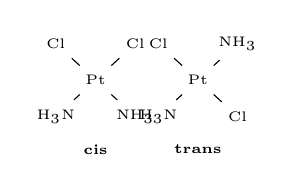
\begin{tikzpicture}[x=4.2mm,y=4.2mm,font=\tiny]
\node (p) at (0,0){Pt}; \node (a) at (-1.2,1.1){Cl}; \node (b) at (1.2,1.1){Cl}; \node (c) at (-1.2,-1.1){H$_3$N}; \node (d) at (1.2,-1.1){NH$_3$};
\foreach \n in {a,b,c,d}{\draw (p)--(\n);} \node at (0,-2.1){\textbf{cis}};
\begin{scope}[xshift=13mm]
\node (p) at (0,0){Pt}; \node (a) at (-1.2,1.1){Cl}; \node (b) at (1.2,1.1){NH$_3$}; \node (c) at (-1.2,-1.1){H$_3$N}; \node (d) at (1.2,-1.1){Cl};
\foreach \n in {a,b,c,d}{\draw (p)--(\n);} \node at (0,-2.1){\textbf{trans}};
\end{scope}
\end{tikzpicture}
\end{minipage}\hfill
\begin{minipage}[c]{0.6\linewidth}\scriptsize
\begin{fl}
\item \textbf{Geometrical}: square planar \ce{[MX2L2]} cis/trans (\ce{[Pt(NH3)2Cl2]}; cis-platin is the anticancer drug). Tetrahedral complexes show \emph{no} geometrical isomerism.
\item Octahedral \ce{[MX2L4]} cis/trans (\ce{[Co(NH3)4Cl2]+}); \ce{[MX3L3]} \textbf{fac/mer} (\ce{[Co(NH3)3(NO2)3]}).
\end{fl}
\end{minipage}
\begin{fl}
\item \textbf{Optical}: non-superimposable mirror images (d/l, dextro/laevo). Common in octahedral complexes with didentate ligands: \ce{[Co(en)3]^3+}, \emph{cis}-\ce{[CoCl2(en)2]+} (the trans form has a plane of symmetry — optically inactive).
\end{fl}
{\scriptsize\setlength{\tabcolsep}{2pt}
\begin{tabularx}{\linewidth}{@{}l l Y@{}}
\toprule
\textbf{Type} & \textbf{Example} & \textbf{Stereoisomers}\\
\midrule
\ce{[MA2B2]} square planar & \ce{[Pt(NH3)2Cl2]} & 2 geometrical (cis, trans); no optical\\
\ce{[MABCD]} square planar & \ce{[Pt(NH3)(Br)(Cl)(py)]} & 3 geometrical\\
\ce{[MA4B2]} octahedral & \ce{[Co(NH3)4Cl2]+} & 2 (cis, trans); no optical\\
\ce{[MA3B3]} octahedral & \ce{[Co(NH3)3(NO2)3]} & 2 (fac, mer); no optical\\
\ce{[M(AA)3]} & \ce{[Co(en)3]^3+}, \ce{[Cr(ox)3]^3-} & 2 optical (d, l)\\
\ce{[M(AA)2B2]} & \ce{[CoCl2(en)2]+} & 3: trans (inactive) + cis-d + cis-l\\
\bottomrule
\end{tabularx}\par}

\chapbar{Bonding I — Valence Bond Theory}
{\scriptsize
\begin{tabularx}{\linewidth}{@{}c l l Y@{}}
\toprule
\textbf{CN} & \textbf{Hybridisation} & \textbf{Shape} & \textbf{Example}\\
\midrule
4 & $sp^3$ & tetrahedral & \ce{[Ni(CO)4]}, \ce{[NiCl4]^2-}, \ce{[CoCl4]^2-}\\
4 & $dsp^2$ & square planar & \ce{[Ni(CN)4]^2-}, \ce{[Pt(NH3)2Cl2]}\\
5 & $sp^3d$ & trigonal bipyramidal & \ce{[Fe(CO)5]}\\
6 & $d^2sp^3$ (inner, $(n-1)d$) & octahedral & \ce{[Co(NH3)6]^3+}, \ce{[Fe(CN)6]^3-}\\
6 & $sp^3d^2$ (outer, $nd$) & octahedral & \ce{[CoF6]^3-}, \ce{[FeF6]^3-}\\
\bottomrule
\end{tabularx}\par}
\vspace{2pt}
{\scriptsize\renewcommand{\arraystretch}{1.3}
\noindent\begin{tabular}{@{}>{\raggedright\arraybackslash}p{0.37\linewidth}@{\ }l@{}}
\ce{[Co(NH3)6]^3+}: Co$^{3+}$ $3d^6$, NH$_3$ pairs → $d^2sp^3$, inner, diamagnetic & \ob{2,2,2,3,3}\,\ob{3}\,\ob{3,3,3}\\
\ce{[CoF6]^3-}: F$^-$ weak, no pairing → $sp^3d^2$, outer, 4 unpaired & \ob{2,1,1,1,1}\,\ob{3}\,\ob{3,3,3}\,\ob{3,3,0,0,0}\\
\ce{[NiCl4]^2-}: Ni$^{2+}$ $3d^8$ → $sp^3$, tetrahedral, 2 unpaired & \ob{2,2,2,1,1}\,\ob{3}\,\ob{3,3,3}\\
\ce{[Ni(CN)4]^2-}: CN$^-$ pairs → $dsp^2$, square planar, diamagnetic & \ob{2,2,2,2,3}\,\ob{3}\,\ob{3,3,0}\\
\end{tabular}\par}
\noindent{\tiny boxes: 3d \;|\; 4s \;|\; 4p \;|\; 4d; shaded = electron pair donated by ligand.}
\begin{fl}
\item \ce{[Ni(CO)4]}: Ni(0) $3d^84s^2$ → $3d^{10}$, $sp^3$, tetrahedral, diamagnetic. \ce{[Fe(CN)6]^3-}: $d^5$ low spin, $d^2sp^3$, 1 unpaired (1.73 BM). \ce{[Fe(CN)6]^4-}: $d^6$, diamagnetic. \ce{[Cr(NH3)6]^3+}: $d^3$, $d^2sp^3$, 3 unpaired. \ce{[Mn(CN)6]^3-}: $d^4$, $d^2sp^3$, 2 unpaired. \ce{[MnCl4]^2-}: $sp^3$, 5 unpaired.
\item \textbf{Limitations of VBT}: many assumptions; no quantitative magnetic data; does not explain colour; no distinction of weak/strong ligands; cannot predict tetrahedral vs square planar for CN 4; no quantitative stability.
\end{fl}

\chapbar{Bonding II — Crystal Field Theory}
\noindent\begin{minipage}[c]{0.55\linewidth}\centering
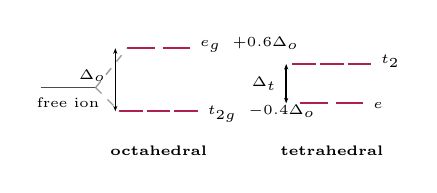
\begin{tikzpicture}[x=1cm,y=1cm,font=\tiny,line width=0.5pt]
\draw[black!70] (0,0.75)--(0.7,0.75); \node[below] at (0.35,0.75){free ion};
\draw[uV,thick] (1.1,1.25)--(1.45,1.25) (1.55,1.25)--(1.9,1.25); \node[right] at (1.9,1.3){$e_g$ \;$+0.6\Delta_o$};
\draw[uV,thick] (1.0,0.45)--(1.3,0.45) (1.35,0.45)--(1.65,0.45) (1.7,0.45)--(2.0,0.45); \node[right] at (2.0,0.42){$t_{2g}$ \;$-0.4\Delta_o$};
\draw[dashed,black!40] (0.7,0.75)--(1.1,1.25) (0.7,0.75)--(1.0,0.45);
\draw[{Stealth[length=2pt]}-{Stealth[length=2pt]}] (0.95,0.45)--(0.95,1.25); \node[left] at (0.95,0.9){$\Delta_o$};
\node at (1.5,-0.05){\textbf{octahedral}};
\begin{scope}[xshift=3.2cm]
\draw[uV,thick] (0.0,1.05)--(0.3,1.05) (0.35,1.05)--(0.65,1.05) (0.7,1.05)--(1.0,1.05); \node[right] at (1.0,1.08){$t_2$};
\draw[uV,thick] (0.1,0.55)--(0.45,0.55) (0.55,0.55)--(0.9,0.55); \node[right] at (0.9,0.52){$e$};
\draw[{Stealth[length=2pt]}-{Stealth[length=2pt]}] (-0.08,0.55)--(-0.08,1.05); \node[left] at (-0.08,0.8){$\Delta_t$};
\node at (0.5,-0.05){\textbf{tetrahedral}};
\end{scope}
\end{tikzpicture}
\end{minipage}\hfill
\begin{minipage}[c]{0.43\linewidth}\scriptsize
\begin{fl}
\item Ligands treated as point charges; d orbitals split.
\item Octahedral: $e_g$ ($d_{x^2-y^2}$, $d_{z^2}$) up; $t_{2g}$ ($d_{xy}$, $d_{yz}$, $d_{xz}$) down.
\item Tetrahedral: inverted; $\Delta_t=\frac49\Delta_o$ → always high spin.
\end{fl}
\end{minipage}
\begin{kbox}
\textbf{Spectrochemical series} (increasing $\Delta_o$):\\
\ce{I-} $<$ \ce{Br-} $<$ \ce{SCN-} $<$ \ce{Cl-} $<$ \ce{S^2-} $<$ \ce{F-} $<$ \ce{OH-} $<$ \ce{C2O4^2-} $<$ \ce{H2O} $<$ \ce{NCS-} $<$ edta$^{4-}$ $<$ \ce{NH3} $<$ en $<$ \ce{CN-} $<$ CO\\[2pt]
$d^4$--$d^7$: $\Delta_o<P$ (weak field) → high spin, e.g.\ $d^4$ = $t_{2g}^3e_g^1$;\quad $\Delta_o>P$ (strong field) → low spin, $d^4$ = $t_{2g}^4e_g^0$\\[1pt]
CFSE (octahedral) $=(-0.4\,n_{t_{2g}}+0.6\,n_{e_g})\,\Delta_o$ \;(+ $P$ for each extra pairing)
\end{kbox}
{\scriptsize\setlength{\tabcolsep}{2pt}
\begin{tabularx}{\linewidth}{@{}l Y Y@{}}
\toprule
 & \textbf{Weak field (high spin)} & \textbf{Strong field (low spin)}\\
\midrule
$d^4$ & $t_{2g}^3e_g^1$, 4 unp. & $t_{2g}^4$, 2 unp.\\
$d^5$ & $t_{2g}^3e_g^2$, 5 unp. (\ce{[FeF6]^3-}) & $t_{2g}^5$, 1 unp. (\ce{[Fe(CN)6]^3-})\\
$d^6$ & $t_{2g}^4e_g^2$, 4 unp. (\ce{[CoF6]^3-}, \ce{[Fe(H2O)6]^2+}) & $t_{2g}^6$, 0 (\ce{[Co(NH3)6]^3+}, \ce{[Fe(CN)6]^4-})\\
$d^7$ & $t_{2g}^5e_g^2$, 3 unp. & $t_{2g}^6e_g^1$, 1 unp.\\
\bottomrule
\end{tabularx}\par}
\begin{fl}
\item \textbf{Colour}: electron jumps $t_{2g}$ → $e_g$ absorbing light of energy $\Delta_o$; complementary colour seen. \ce{[Ti(H2O)6]^3+} ($d^1$) violet. Anhydrous CuSO$_4$ is white, CuSO$_4$·5H$_2$O blue — no ligands, no splitting. Adding en to green \ce{[Ni(H2O)6]^2+} gives blue → violet \ce{[Ni(en)3]^2+} (larger $\Delta_o$, absorbs shorter $\lambda$). Ruby: Cr$^{3+}$ in Al$_2$O$_3$; emerald: Cr$^{3+}$ in beryl.
\item Stronger ligand → larger $\Delta_o$ → absorbs higher energy (shorter $\lambda$).
\item \textbf{Limitations of CFT}: treats ligands as point charges, so anionic ligands should split most — yet they are at the weak end; ignores covalent character of M--L bonds.
\end{fl}

\chapbar{Metal carbonyls}
\begin{fl}
\item \ce{[Ni(CO)4]} tetrahedral; \ce{[Fe(CO)5]} trigonal bipyramidal; \ce{[Cr(CO)6]} octahedral; \ce{[Mn2(CO)10]} two square pyramids joined by Mn--Mn; \ce{[Co2(CO)8]} Co--Co bond bridged by two CO.
\item \textbf{Synergic bonding}: $\sigma$ bond — lone pair of C → vacant metal orbital; $\pi$ back-bond — filled metal d → vacant antibonding $\pi^*$ of CO. Each strengthens the other: M--C bond strengthens, C--O bond weakens.
\end{fl}

\chapbar{Importance \& applications}
{\scriptsize
\begin{tabularx}{\linewidth}{@{}l Y@{}}
\toprule
Qualitative analysis & Ni$^{2+}$ + dimethylglyoxime → red precipitate; colour reactions of Cu$^{2+}$, Fe$^{3+}$, etc.\\
Hardness of water & titration with Na$_2$EDTA (stable Ca$^{2+}$/Mg$^{2+}$ complexes)\\
Metallurgy & Ag, Au leached as \ce{[Ag(CN)2]-}, \ce{[Au(CN)2]-}; Ni purified via \ce{[Ni(CO)4]} (Mond process)\\
Biology & chlorophyll (Mg), haemoglobin (Fe), vitamin B$_{12}$ cyanocobalamin (Co)\\
Catalysis & Wilkinson's catalyst \ce{[(Ph3P)3RhCl]} — hydrogenation of alkenes\\
Electroplating & smooth Ag/Au coats from \ce{[Ag(CN)2]-}, \ce{[Au(CN)2]-}\\
Photography & hypo dissolves AgBr as \ce{[Ag(S2O3)2]^3-}\\
Medicine & cis-platin (anticancer); EDTA (lead poisoning); D-penicillamine, desferrioxamine B (excess Cu, Fe)\\
\bottomrule
\end{tabularx}\par}
\vspace{2pt}
\begin{numbox}{\sffamily\bfseries\scriptsize\color{uc}STANDARD QUESTION RECIPES\;}\par\scriptsize
\textbf{(1) Hybridisation, shape, magnetism from a formula.} OS of metal → $d^n$ → ligand strong or weak (series) → pair up if strong (CN$^-$, CO, en, NH$_3$ with Co$^{3+}$) → count empty orbitals → hybridisation → shape → unpaired $n$ → $\mu=\sqrt{n(n+2)}$.\\[1pt]
\textbf{(2) $\mu$ given, find $n$.} 1.73→1, 2.83→2, 3.87→3, 4.90→4, 5.92→5. E.g.\ Fe$^{2+}$ complex with 4.90 BM → high spin, outer orbital.\\[1pt]
\textbf{(3) Name ↔ formula.} Charges first, then alphabetical ligands, then OS; check ``-ate'' for anions.\\[1pt]
\textbf{(4) Count ions / AgCl.} Only ions outside [ ] ionise. 1 mol \ce{[CoCl(NH3)5]Cl2} + excess AgNO$_3$ → 2 mol AgCl.\\[1pt]
\textbf{(5) Draw isomers.} Octahedral: put identical ligands at 90$^\circ$ (cis) or 180$^\circ$ (trans); check mirror image for en complexes.\\[1pt]
\textbf{(6) $3d^n$ in $t_{2g}$/$e_g$} and CFSE for weak vs strong field; which absorbs at longer $\lambda$ (weaker ligand).
\end{numbox}
\begin{tip}\Tip Ni$^{2+}$ with CN$^-$ is square planar ($dsp^2$), with Cl$^-$ tetrahedral ($sp^3$). NH$_3$ behaves as strong field with Co$^{3+}$ but \ce{[Ni(NH3)6]^2+} is $sp^3d^2$ (only 2 unpaired either way). $d^3$ (Cr$^{3+}$) is always inner orbital $d^2sp^3$. Tetrahedral complexes: no geometrical isomers, almost always high spin.\end{tip}
\end{multicols}

% ================= CHECKLIST =================
\begin{tcolorbox}[enhanced,colback=navy,colframe=navy,arc=2pt,left=6pt,right=6pt,top=2pt,bottom=2pt,before skip=4pt]
\color{white}\sffamily\bfseries\small BOARD CHECKLIST — Inorganic Chemistry \hfill\footnotesize\mdseries tick when practised ☐
\end{tcolorbox}
\begin{multicols}{2}\raggedcolumns
\scriptsize
\textbf{\textcolor{uIV}{Ch 4 d- \& f-Block}} Configurations incl.\ Cr, Cu and ions; definition of transition element (Zn/Cd/Hg vs Cu/Ag/Au); trends with reasons: m.p./$\Delta_aH$, radii, IE, oxidation states, $E^\circ$ anomalies (Cu, Mn, Zn), Mn$^{3+}$/Cr$^{2+}$, Cu$^+$ disproportionation; colour, magnetism ($\mu$), complexes, catalysis, interstitial compounds, alloys; K$_2$Cr$_2$O$_7$ and KMnO$_4$ preparation and \emph{ionic equations}; lanthanoid contraction + consequences; lanthanoids vs actinoids table; Mischmetall.

\textbf{\textcolor{uV}{Ch 5 Coordination}} Werner's postulates and the CoCl$_3$·$x$NH$_3$ series; double salt vs complex; definitions (ligand types, ambidentate, chelate, CN, homo/heteroleptic); IUPAC names both ways; structural and stereo isomers with drawings; VBT for the eight standard complexes; CFT splitting diagrams, spectrochemical series, high/low spin, $t_{2g}/e_g$ configuration, colour; limitations of VBT and CFT; synergic bonding; applications.
\end{multicols}

\begin{tcolorbox}[enhanced,colback=white,colframe=navy,boxrule=0.8pt,arc=2pt,title={\sffamily\bfseries\footnotesize My notes},colbacktitle=navy,coltitle=white,height fill,before skip=4pt]
\end{tcolorbox}
\end{document}
